\subsection{Memory}\label{subsec: processor-memory}
OlaVM的内存设计为可随机访问为的读写模式。对其约束也是按照该模式进行设计。读写内存地址的值通过将地址存入寄存器,之后通过 $\texttt{[r}_n\texttt{]}$ 来进行读写操作。
Memory的结构采用B-Tree模式。可以通过地址随机寻址,读取和写入数据到Memory。B-Tree的优点插入数据时按照地址进行了排序。因此在下边两个场景下提高了效率。
\begin{enumerate}
    \item 随机读内存地址数据数据,根据内存地址通过B-tree数据结构快速找到地址下存的数据。
    \item 根据内存地址和clk排序生成memory trace table时,顺序在插入时已排好,可以直接顺序处理,不用再次排序。
\end{enumerate}

下图是内存数据结构的示意图\ref{fig: B-tree-memory}:
\begin{figure}[!htp]
    \centering
    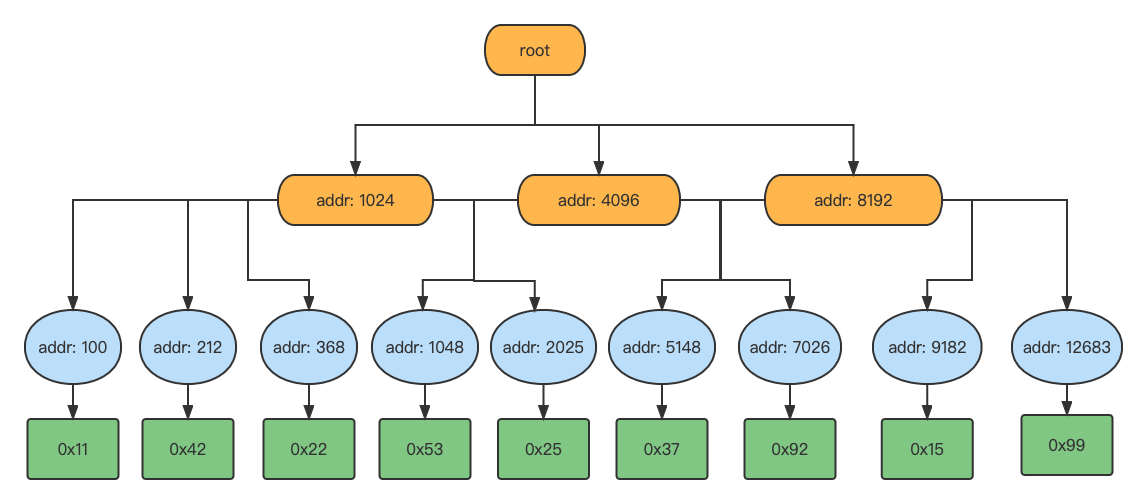
\includegraphics[width=0.8\textwidth]{b_tree_hash}
    \caption{OlaVM memory存储数据结构}
    \label{fig: B-tree-memory}
\end{figure}